\documentclass[12pt]{article}

\usepackage[utf8]{inputenc} % important for pdflatex + any UTF-8 characters
\usepackage{amsmath, amssymb}
\usepackage{geometry}
\geometry{margin=1in}
\usepackage{graphicx}
\setlength{\parindent}{0pt}

\title{Solutions -- Practice Problem Set 1}
\author{ECON 300 -- Labour Economics}
\date{Winter 2026}

\begin{document}
\maketitle

\subsection*{Problem 1: Labour Force Participation (Solution)}

\textbf{Given:}
\[
\text{Working-age population} = 800{,}000,\quad E = 520{,}000,\quad U = 40{,}000,\quad N = 240{,}000
\]
where $E$ = employed, $U$ = unemployed, $N$ = not in labour force.

\begin{enumerate}
\item \textbf{Labour force.} The labour force is employed plus unemployed:
\[
LF = E + U = 520{,}000 + 40{,}000 = 560{,}000.
\]

\item \textbf{Labour force participation rate (LFPR).}
\[
LFPR = \frac{LF}{\text{Working-age population}} = \frac{560{,}000}{800{,}000} = 0.70 = 70\%.
\]

\item \textbf{Unemployment rate.}
\[
u = \frac{U}{LF} = \frac{40{,}000}{560{,}000} = 0.071428\ldots \approx 7.14\%.
\]

\item \textbf{Employment-to-population ratio.}
\[
\frac{E}{\text{Working-age population}} = \frac{520{,}000}{800{,}000} = 0.65 = 65\%.
\]

\item \textbf{Interpretation.} The LFPR (70\%) measures the share of working-age people who are \emph{in the labour force} (working or actively searching). The employment-to-population ratio (65\%) measures the share who are \emph{actually employed}. The gap (70\% -- 65\% = 5 percentage points) reflects unemployment among labour force participants.
\end{enumerate}

\subsection*{Problem 2: Labour Supply and the Reservation Wage (Solution)}

\textbf{Given budget constraint:}
\[
C = 500 + 20h
\]
\textbf{Utility:}
\[
U = C - 0.5h^2
\]

\begin{enumerate}
\item \textbf{Derive the labour supply function.}

Substitute the budget constraint into utility:
\[
U(h) = (500 + 20h) - 0.5h^2 = 500 + 20h - 0.5h^2.
\]

Maximize $U(h)$ with respect to $h$.

Compute the first derivative:
\[
\frac{dU}{dh} = 20 - h.
\]

Set FOC to zero:
\[
20 - h = 0 \quad \Rightarrow \quad h^* = 20.
\]

Second derivative:
\[
\frac{d^2U}{dh^2} = -1 < 0,
\]
so this is a maximum.

\textbf{Labour supply at wage \$20/hour is $h^*=20$ hours.}

\item \textbf{Optimal hours worked.} From above:
\[
h^* = 20.
\]

\item \textbf{Reservation wage.}

To define the reservation wage, it is helpful to write the model with a general wage $w$:
\[
C = 500 + wh.
\]
Then:
\[
U(h) = 500 + wh - 0.5h^2.
\]
FOC:
\[
\frac{dU}{dh} = w - h = 0 \quad \Rightarrow \quad h^*(w) = w.
\]

The reservation wage is the wage at which the worker is just indifferent between working a (marginal) hour and not working. In this model, the interior solution implies:
\[
h^*(w) = 0 \iff w = 0.
\]
So the reservation wage is:
\[
w^R = 0.
\]

\item \textbf{Economic meaning.} The reservation wage is the minimum wage required for the worker to supply positive hours of work. Here, because utility increases with consumption and the marginal disutility of work at $h=0$ is zero, any positive wage induces some work. In more realistic settings (fixed costs of working, commuting, childcare, or stronger preference for leisure), the reservation wage would be strictly positive.
\end{enumerate}

\subsection*{Problem 3: Income and Substitution Effects (Solution)}

\textbf{Given:} initial wage $w_0=\$25$, new wage $w_1=\$30$, hours initially $h_0=40$.

\begin{enumerate}
\item \textbf{Change in weekly income (holding hours fixed at 40).}

Initial weekly earnings:
\[
Y_0 = 25 \times 40 = 1000.
\]
New weekly earnings:
\[
Y_1 = 30 \times 40 = 1200.
\]
Change:
\[
\Delta Y = Y_1 - Y_0 = 1200 - 1000 = 200.
\]
So weekly income increases by \textbf{\$200} (if hours stayed at 40).

\item \textbf{Explain substitution and income effects.}

\begin{itemize}
\item \textbf{Substitution effect:} A higher wage increases the opportunity cost of leisure (each hour of leisure now ``costs'' more foregone earnings). This makes leisure relatively more expensive and tends to \emph{reduce leisure}, which tends to \emph{increase hours worked}.

\item \textbf{Income effect:} A higher wage raises income for any given number of hours worked. If leisure is a normal good, higher income increases the demand for leisure, which tends to \emph{increase leisure} and \emph{reduce hours worked}.
\end{itemize}

The net change in hours depends on which effect dominates.

\item \textbf{When could hours worked fall after a wage increase?}

Hours worked could fall if the \textbf{income effect dominates} the substitution effect. This is more likely when:
\begin{itemize}
\item the worker is already working many hours (marginal disutility of work is high), and/or
\item preferences place a high value on leisure, and/or
\item the wage is high enough that the worker can maintain consumption goals with fewer hours.
\end{itemize}
In that case, labour supply can be \textbf{backward-bending} over some range.
\end{enumerate}

\subsection*{Problem 4: Labour Supply and Leisure (Graphical Analysis) (Solution)}

\textbf{Set-up (standard labour--leisure model).} Let total available time be $T$ hours per week, leisure be $L$, and hours worked be $h=T-L$.

With non-labour income $V$ and wage $w$, consumption is:
\[
C = V + w(T-L).
\]
This is a straight line in $(L,C)$ space with:
\[
\text{slope} = -w,\quad C\text{-intercept} = V + wT,\quad L\text{-intercept} = T.
\]

\begin{enumerate}
\item \textbf{Budget constraint at $w=\$20$.} The budget line has slope $-20$. Compared to a lower wage, it is steeper in absolute value.

\item \textbf{Budget constraint at $w=\$30$.} The budget line has slope $-30$ and pivots upward around $L=T$ (the leisure intercept does not change, since $h=0$ implies $L=T$ regardless of wage).

\item \textbf{Substitution vs income effect (graphical).}
\begin{itemize}
\item The wage increase makes the budget line steeper $\Rightarrow$ leisure is more expensive $\Rightarrow$ substitution effect reduces leisure (increases hours).
\item The wage increase raises attainable consumption $\Rightarrow$ if leisure is normal, income effect increases leisure (reduces hours).
\end{itemize}
A standard decomposition uses a compensated (Hicks) budget line tangent to the original indifference curve to isolate the substitution effect, and then the shift from compensated to new optimum is the income effect.

\item \textbf{Reservation wage on the graph.} The reservation wage is the slope magnitude at which the worker is just indifferent between working and not working. Graphically, it is the wage where an indifference curve at the endowment point $(L=T, C=V)$ is just tangent to the budget line. If market wage is below $w^R$, optimal choice is $h=0$ (all leisure).
\end{enumerate}




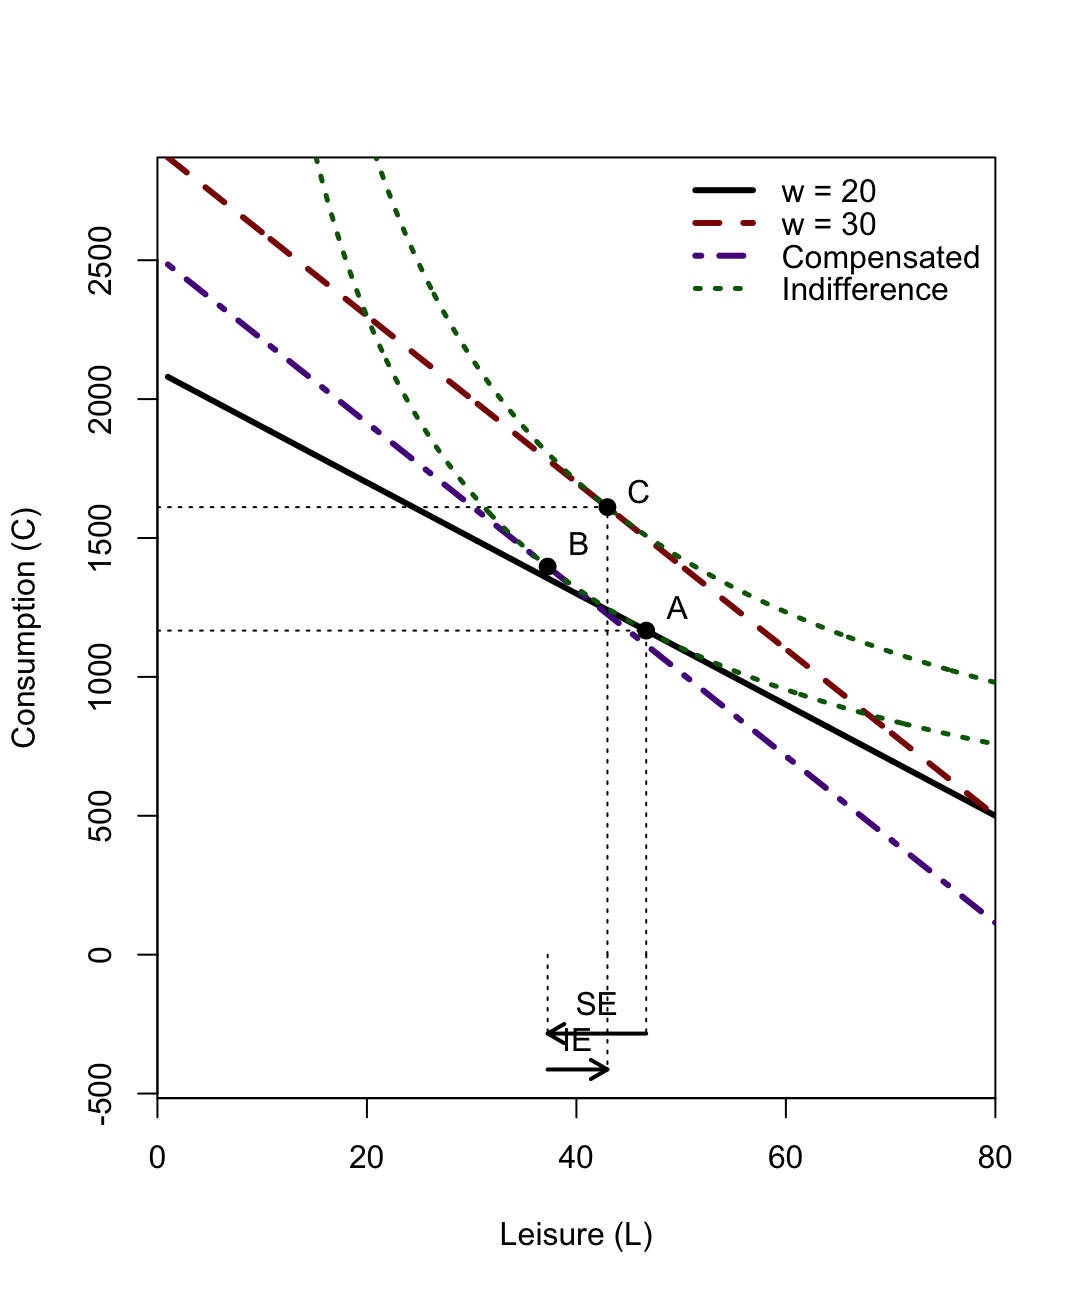
\includegraphics[width=1.1\linewidth]{P4_diagram.png}



\subsection*{Problem 5: Market Labour Supply and Demand (Solution)}

\textbf{Given:}
\[
L^D = 100 - 2w,\qquad L^S = 20 + 3w.
\]

\begin{enumerate}
\item \textbf{Equilibrium wage and employment.}

Set demand equal to supply:
\[
100 - 2w = 20 + 3w \quad \Rightarrow \quad 80 = 5w \quad \Rightarrow \quad w^* = 16.
\]
Equilibrium employment:
\[
L^* = 100 - 2(16) = 100 - 32 = 68.
\]
(Checks with supply: $20 + 3(16)=20+48=68$.)

\item \textbf{Graph.} Labour demand is downward sloping and labour supply upward sloping. Their intersection occurs at $(L,w)=(68,16)$.

\item \textbf{Minimum wage $w_m=\$18$.}

Since $18 > 16$, the minimum wage is \textbf{binding}.

Employment is determined by labour demand at $w=18$:
\[
L^D(18) = 100 - 2(18) = 100 - 36 = 64.
\]
Labour supplied at $w=18$:
\[
L^S(18) = 20 + 3(18) = 20 + 54 = 74.
\]
Unemployment (excess supply):
\[
U = L^S - L^D = 74 - 64 = 10.
\]

\item \textbf{Economic intuition.} A binding minimum wage raises the wage above equilibrium. Firms reduce hiring (move along labour demand), while more workers are willing to work (move along labour supply). The difference between workers who want jobs and jobs offered is unemployment.
\end{enumerate}

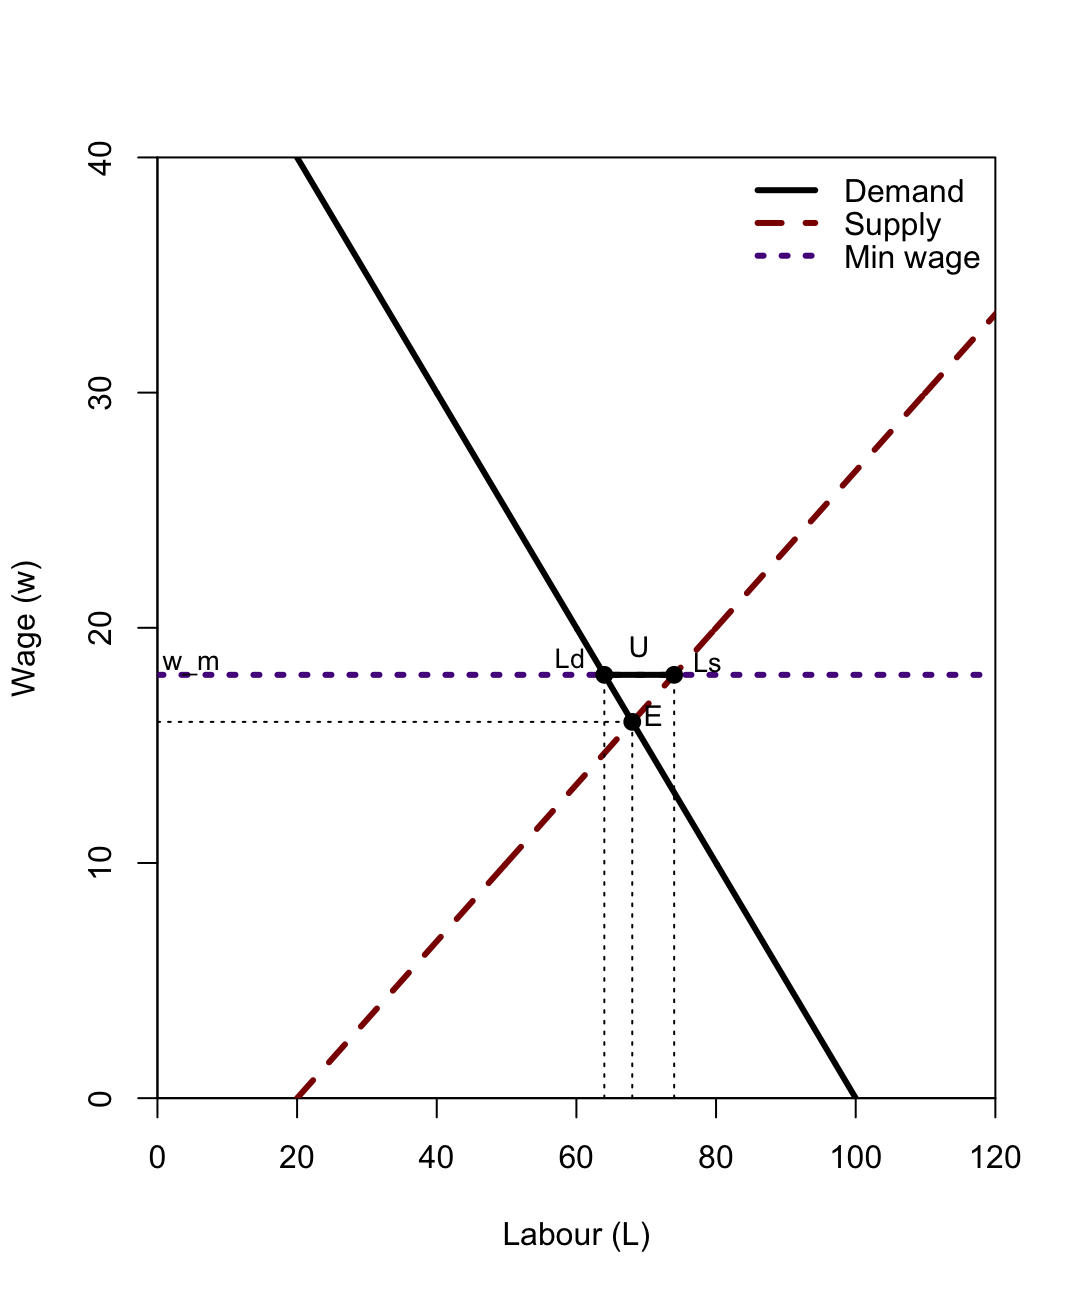
\includegraphics[width=1.1\linewidth]{P5_diagram.png}


\end{document}